\section{Apprendice}
%------------------------------------------------

\begin{frame}[plain]
	\begin{center}
		{\Huge Appendici varie della presentazione}
	\end{center}
\end{frame}

\begin{frame}
	\frametitle{Secure Hash Algorithm: Iterazioni}

	Ogni iterazione usa una funzione non lineare (\textit{f}) e una costante (\textit{k}) che varia a seconda dell'intervallo di iterazione.
	La costante k viene successivamente utilizzata all'interno della funzione di compressione.

	\begin{itemize}
		\item \textbf{Iterazioni 0-19}: \textit{f = (b and c) or (not b and d)} con \textit{k = 0x5A827999}
		\item \textbf{Iterazioni 20-39}: \textit{f = b xor c xor d} con \textit{k = 0x6ED9EBA1}
		\item \textbf{Iterazioni 40-59}: \textit{f = (b and c) or (b and d) or (c and d)} con \textit{k = 0x8F1BBCDC}
		\item \textbf{Iterazioni 60-79}: \textit{f = b xor c xor d} con \textit{k = 0xCA62C1D6}
	\end{itemize}

\end{frame}

\begin{frame}
	\frametitle{Quali utilizzi ci sono per le funzioni hash}
	\begin{itemize}
		\item \textbf{Message fingerprint}(Integrità dei dati)
		\item \textbf{Password hashing}(Database di password)
		\item \textbf{Entity Authentication/Identification}(meccanismo challenge-response prevenire impersonificazione)
		\item \textbf{Message Authentication} (MAC)
		\item \textbf{Encryption} (pseudorandom bit stream)
	\end{itemize}
\end{frame}

\begin{frame}
	\frametitle{Message Authentication Code (MAC)}

	Il MAC (Message Authentication Code) è simile a una firma digitale.
	Quando si riceve un messaggio, si eseguono delle computazioni sul messaggio ricevuto e \textbf{si confronta il risultato con il MAC ricevuto}.

	\begin{itemize}
		\item Conoscendo il MAC di un messaggio, è impossibile generare un altro messaggio con lo stesso MAC.
		\item È impossibile trovare due messaggi con lo stesso MAC.
		\item I MAC sono distribuiti uniformemente.
		\item Il MAC deve dipendere da ogni bit del messaggio.
	\end{itemize}
\end{frame}

\begin{frame}
	\frametitle{H-MAC}

	MAC viene generato tramite un meccanismo di crittografia simmetrica, ma esistono anche soluzioni come H-MAC
	che sfruttano una funzione hash.

	\vspace{1cm}

	H-MAC esegue una funzione di hash due o tre volte a partire da una stessa chiave. In teoria, H-MAC potrebbe essere
	calcolato con qualsiasi funzione hash, anche se in pratica si utilizzano quasi sempre \textbf{SHA-1 o MD5 (entrambi obsoleti)}.


\end{frame}

\begin{frame}
	\frametitle{H-MAC Parte 2}

	H-MAC viene calcolato a blocchi e a seconda della chiave K bisognerà adattarla alla lunghezza del blocco.

	\[
		\text{H-MAC}(K, M') = H((K' \oplus \text{opad}) \| H((K' \oplus \text{ipad}) \| M'))
	\]

	Dove $K'$ è la chiave $\text{opad}$/$\text{ipad}$ sono costanti.

\end{frame}

\begin{frame}
	\frametitle{Generazione della Firma Digitale con PGP}

	\begin{columns}
		% Colonna a sinistra (Testo)
		\begin{column}{0.4\textwidth}
			PGP calcola un hash dal testo in chiaro, e crea poi da questo hash la firma digitale usando la \textbf{chiave privata del mittente}.
		\end{column}

		% Colonna a destra (Immagine)
		\begin{column}{0.6\textwidth}
			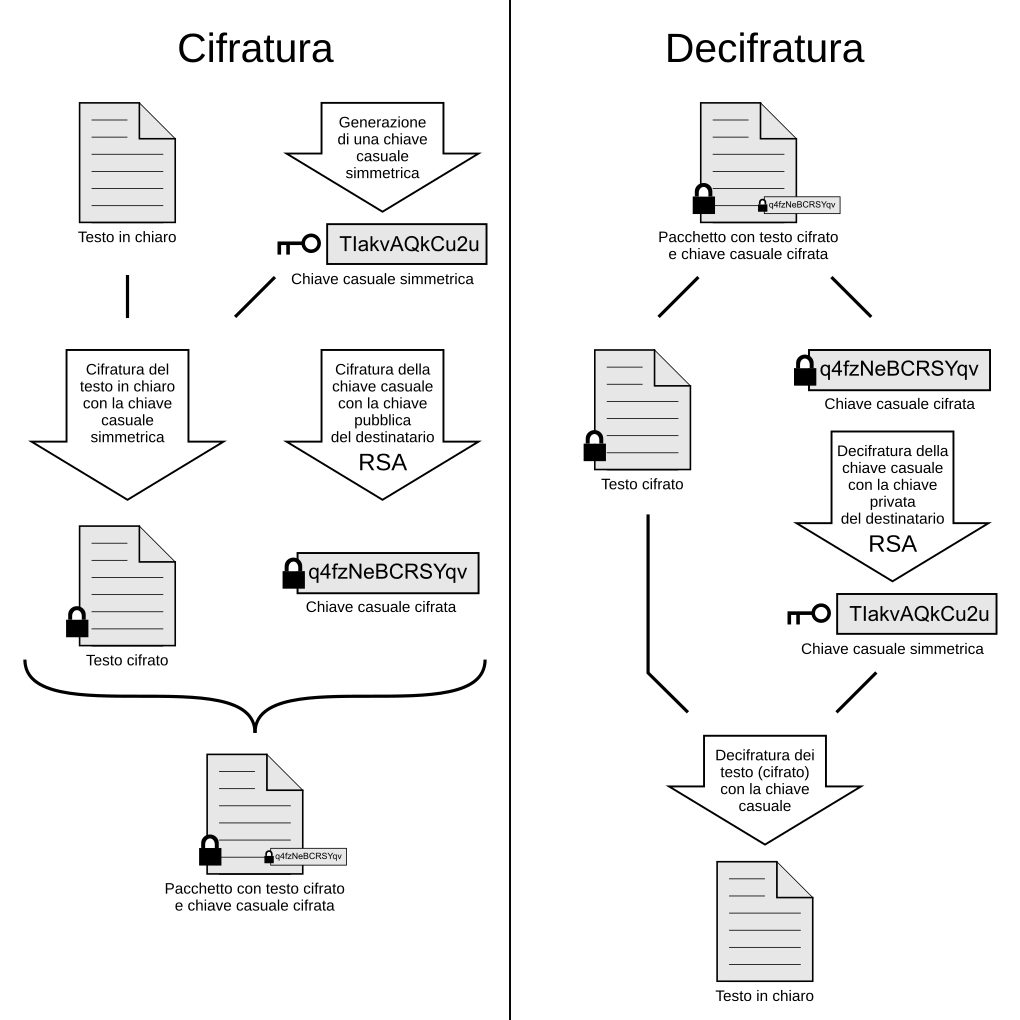
\includegraphics[width=\textwidth]{img/1-img/PGP_diagram_IT.png}
		\end{column}
	\end{columns}

\end{frame}


\begin{frame}
	\frametitle{Verifica della Firma Digitale con PGP}

	\begin{columns}
		% Colonna a sinistra (Testo)
		\begin{column}{0.4\textwidth}
			Il destinatario del messaggio calcola il message digest dal testo in chiaro decifrato, e poi usa la \textbf{chiave pubblica del mittente} per decifrare la firma digitale. \\
			Si può verificare la non alterazione del messaggio e l'autenticità del mittente.
		\end{column}

		% Colonna a destra (Immagine)
		\begin{column}{0.6\textwidth}
			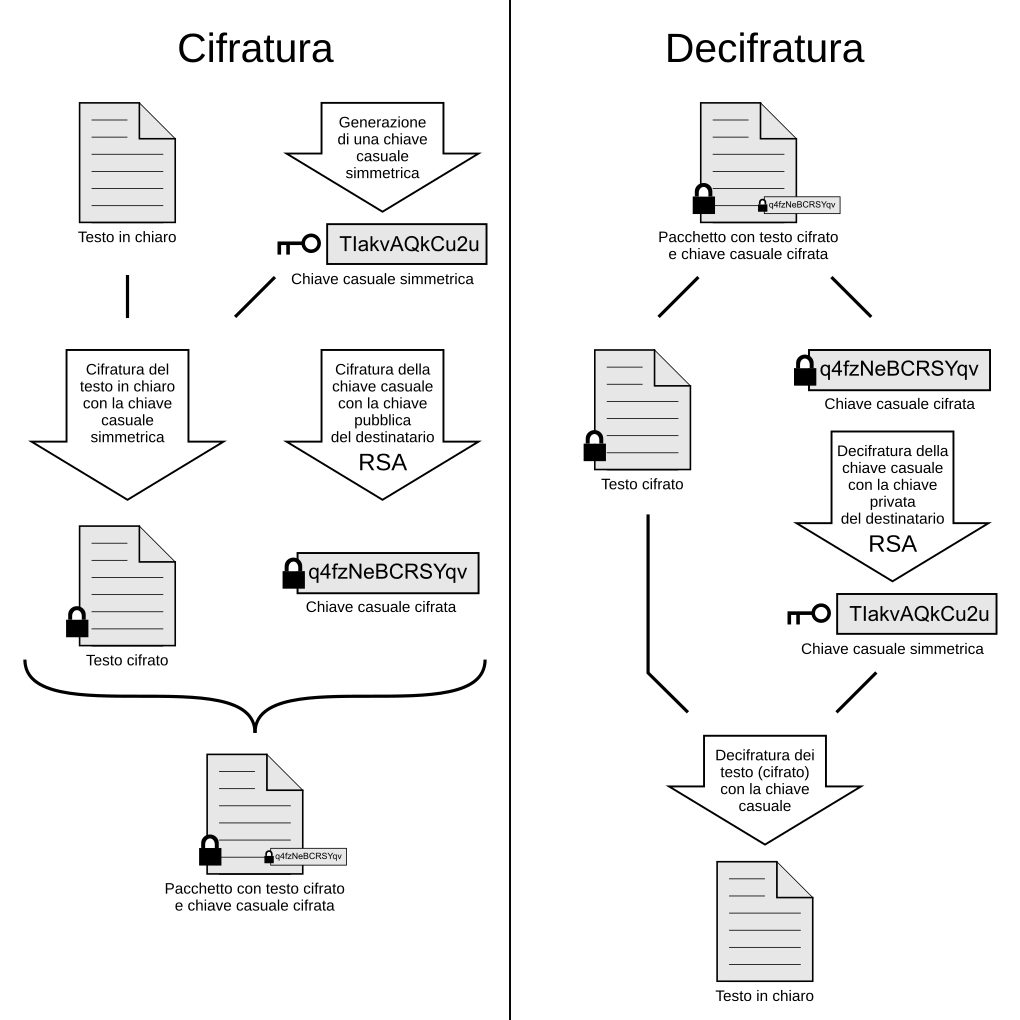
\includegraphics[width=\textwidth]{img/1-img/PGP_diagram_IT.png}
		\end{column}
	\end{columns}

\end{frame}



\begin{frame}
	\frametitle{Blocco finale di SHA-1}
	\begin{center}
		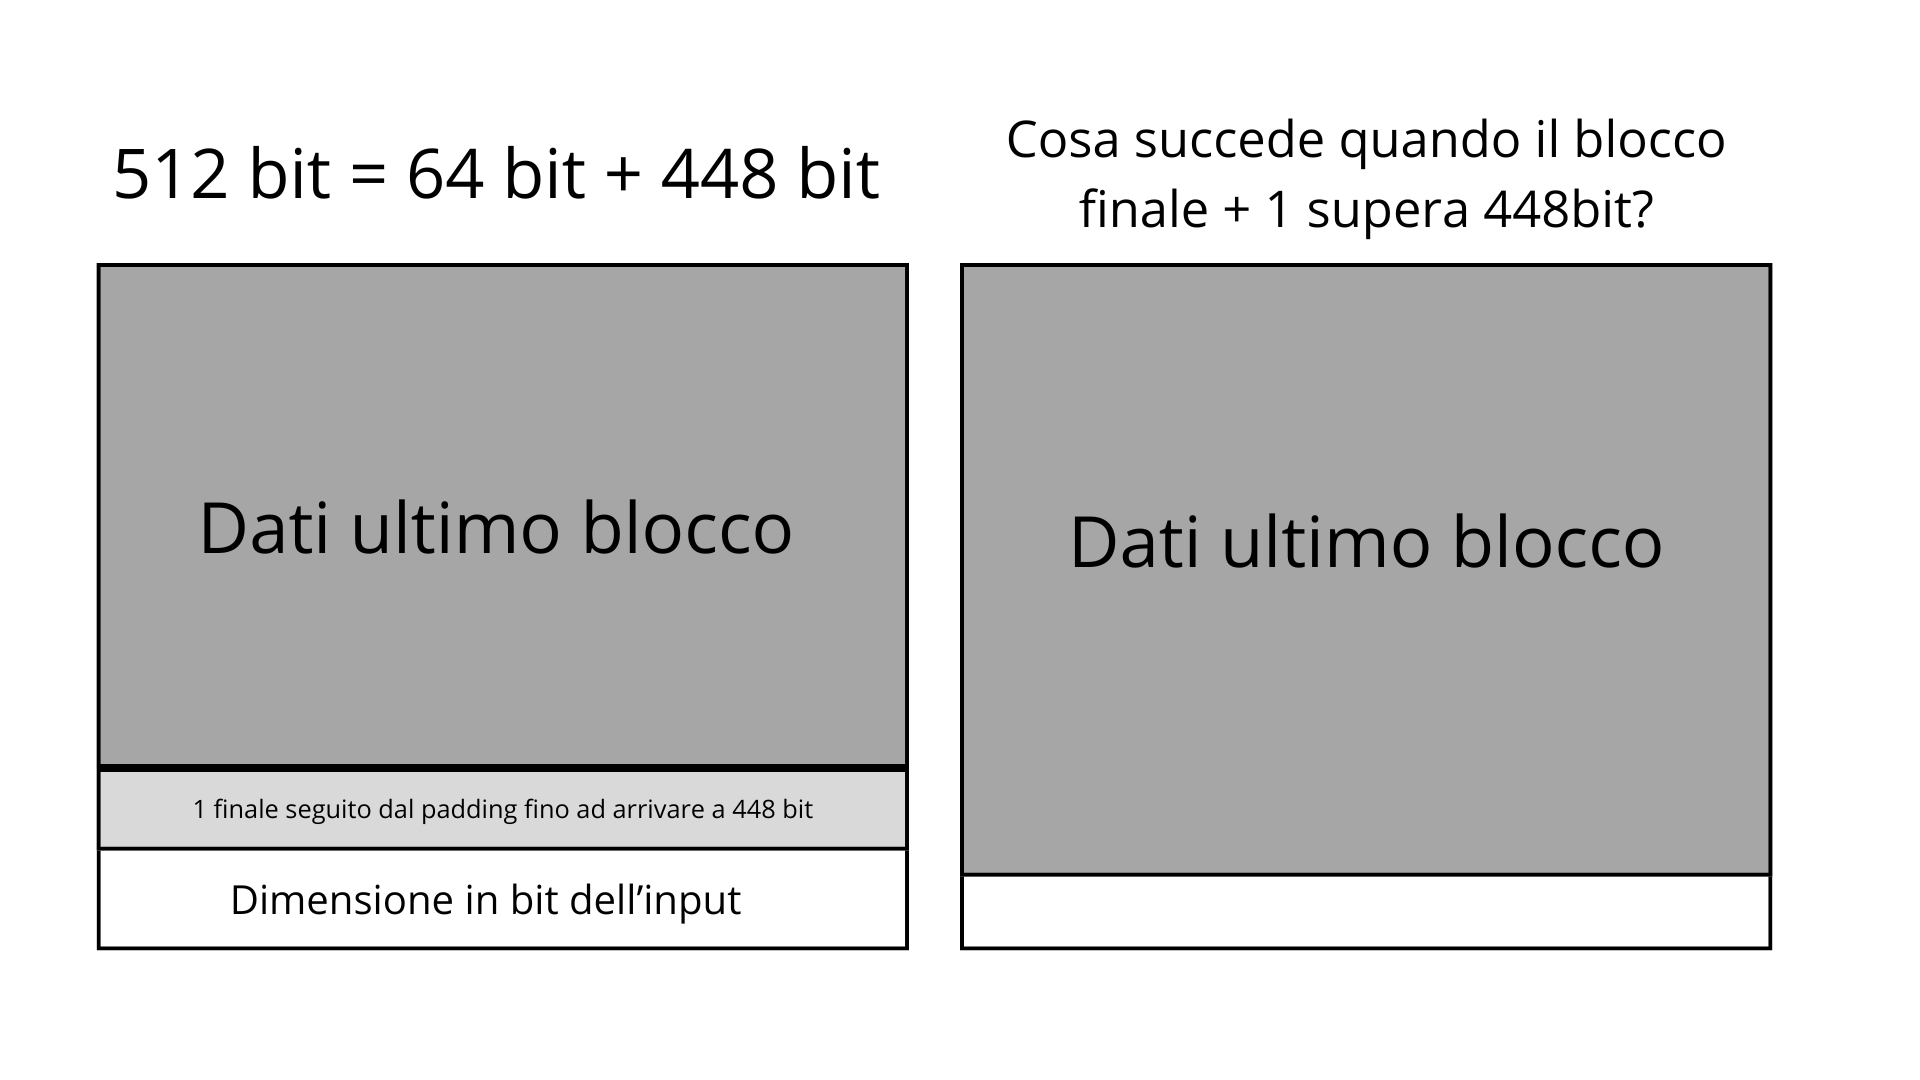
\includegraphics[width=1\textwidth]{img/3-img/blocco-finale1.png}
	\end{center}

\end{frame}

\begin{frame}
	\frametitle{Blocco finale di SHA-1 Soluzione}
	\begin{center}
		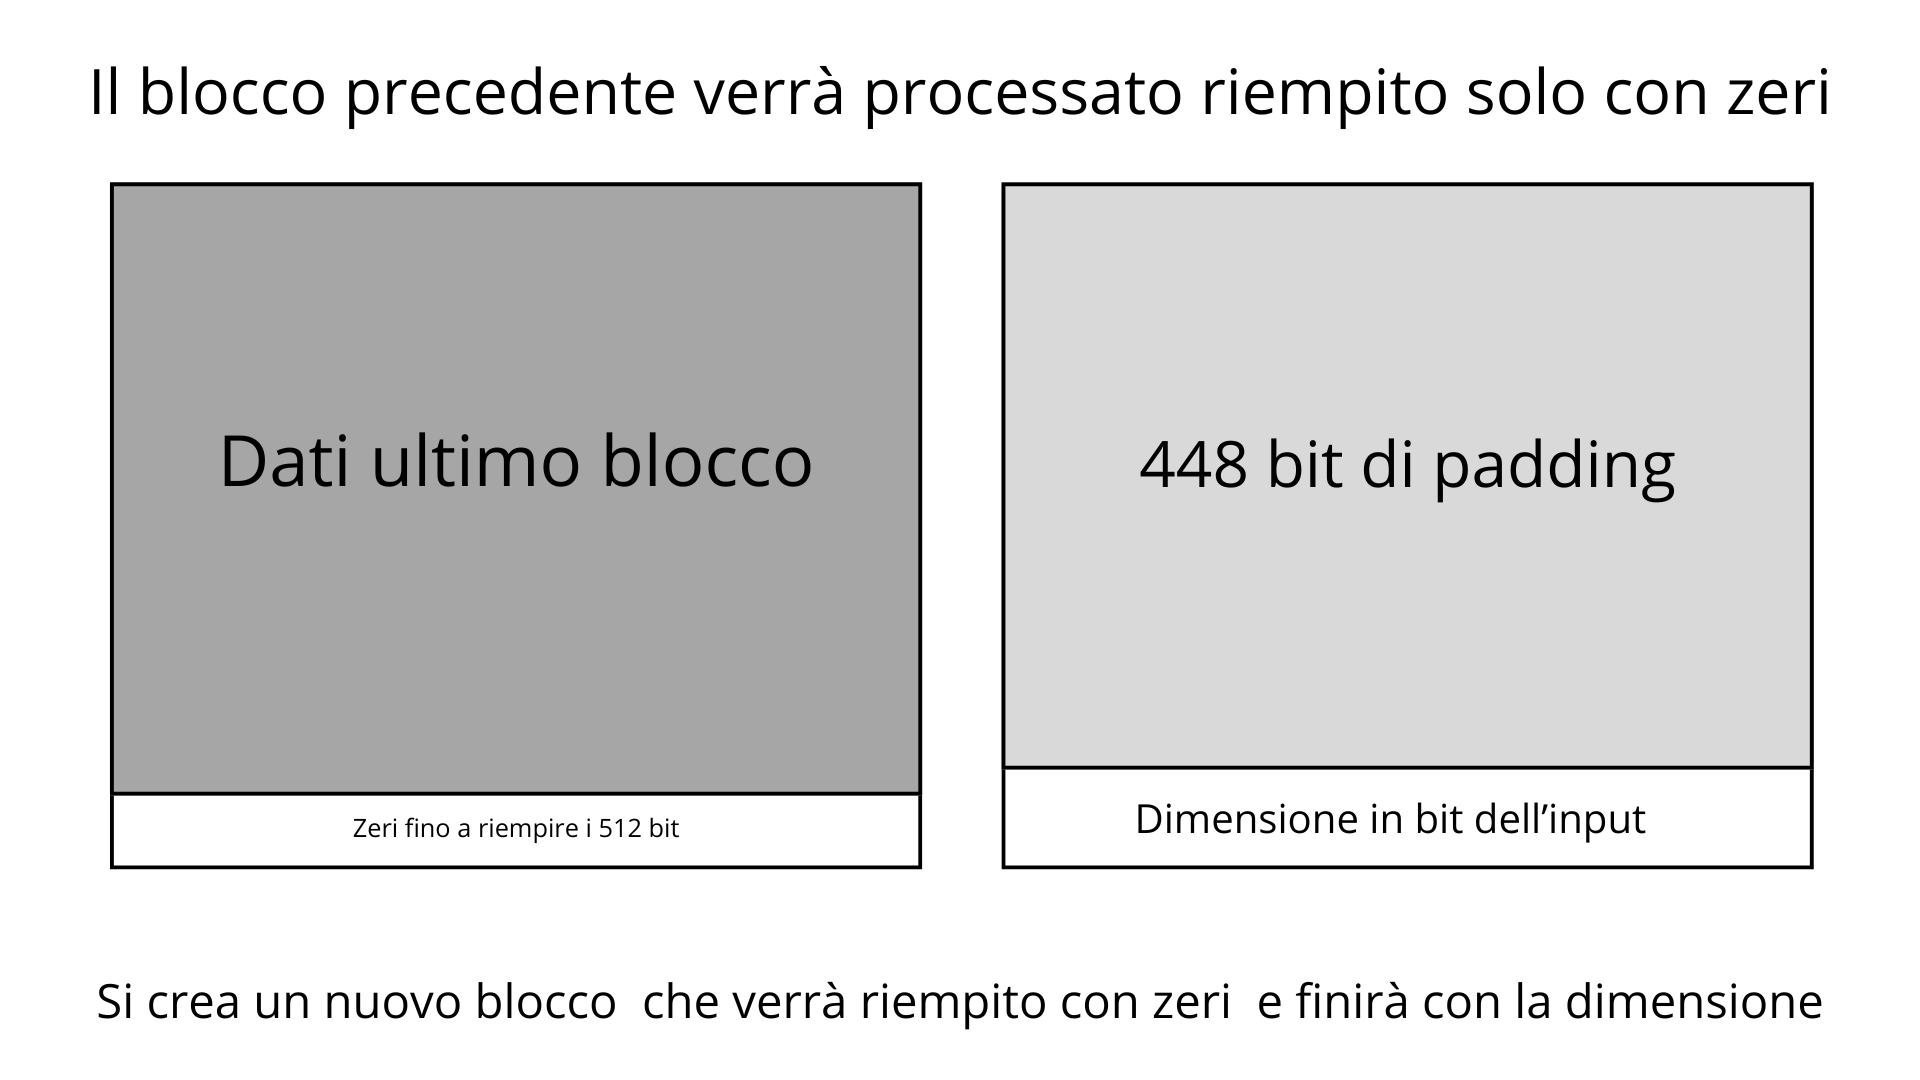
\includegraphics[width=1\textwidth]{img/3-img/blocco-finale2.png}
	\end{center}

\end{frame}



\begin{frame}[fragile]
	\frametitle{Rotazione a sinistra}
	Operazione che ha il compito di \textbf{espandere le parole} all'interno dell'algoritmo.
	La differenza tra SHA-1 e SHA-0 è una rotazione a sinistra di 1 bit.

	\vspace{1cm}

	\begin{verbatim}
	retuen type-> uint32_t 
	
	leftRotate(uint32_t value, unsigned int count) 
	{
	return (value << count) | (value >> (32 - count));
	}
    \end{verbatim}
\end{frame}

\begin{frame}[fragile]
	\frametitle{Esempio con un numero a 8 bit}

	Rotazione di 3 bit a sinistra di un numero a 8 bit.

	\begin{verbatim}

	Valore iniziale:    		
	10110101

	-> Shift a Sx di 3 bit:
	10101xxx
	
	-> Shift a Dx di (8-3) bit:
	00000101

	Concateno i due risultati: 10101|101
	
	\end{verbatim}
\end{frame}